\documentclass[dvips, intlimits, 9pt, unicode, notheorems]{beamer}
\usepackage[russian]{babel}
\usepackage{beamerthemesplit}
\usepackage[T1,T2A]{fontenc}
\usepackage[utf8x]{inputenc}
\usepackage{amsthm}
\usepackage{amssymb}
\usepackage{float}
\usepackage{graphicx}
\usepackage{algorithm}
\usepackage{algorithmic}
\usepackage{color}
\usepackage{array}
\usepackage{ulem}

\graphicspath{{../figures/eps/bw/}}

\def\figureref#1{Рис.\,\protect\ref{#1}}
\def\eqref#1{(\protect\ref{#1}\protect)}

\def\putGen#1{\raise-5mm\hbox{\includegraphics[origin=c, scale=0.7]{border-deletion-sequence-#1.eps}}}
\def\putDC#1{\raise-11mm\hbox{\includegraphics[scale=0.8]{tangle-decomp-example-#1.eps}}}

\floatname{algorithm}{Алгоритм}
\theoremstyle{plain}
\newtheorem{theorem}{Теорема}
\newtheorem{lemma}{Лемма}
\theoremstyle{definition}
\newtheorem{definition}{Определение}

\usetheme{Warsaw}

\setbeamerfont{institute}{size=\normalsize}
\setbeamercolor{bluetext_color}{fg=blue}
\newcommand{\bluetext}[1]{{\usebeamercolor[fg]{bluetext_color}#1}}

\title{ Алгоритмическое перечисление альтернированных $k$-танглов }
\author{Мишунин Александр Сергеевич, гр. 602}
\institute{
	УЧРЕЖДЕНИЕ РОССИЙСКОЙ АКАДЕМИИ НАУК САНКТ-ПЕТЕРБУРГСКИЙ АКАДЕМИЧЕСКИЙ УНИВЕРСИТЕТ –-
	НАУЧНО-ОБРАЗОВАТЕЛЬНЫЙ ЦЕНТР НАНОТЕХНОЛОГИЙ РАН \\
	\vspace{0.7cm}
	Научный руководитель:  д. ф. - м. н., Омельченко А. В. \\
	Рецензент: к. ф. - м. н., Мешков В. Р. \\
	\vspace{0.7cm}
}
\date{ Санкт-Петербург \\ 2010 г. }

\begin{document}
	\Russian

	\begin{frame}
		\maketitle
	\end{frame}

	\begin{frame}
		\frametitle{Основные определения}

		\begin{definition}
			\label{definition:tangle}
			$k$-танглом называется гладкое вложение $k$ отрезков и конечного числа окружностей в $B^3$
			(трехмерный замкнутый шар единичного радиуса), если $2k$ концов отрезков взаимно однозначно отображаются
			на точки с координатами $(\cos\pi i/k, \sin\pi i/k, 0)$, $i\in\{0, 1, \dots, 2k{-}1\}$, называемые
			концами $k$-тангла, и больше ни какие точки отрезков или окружностей на границу $B^3$ не отображаются.
		\end{definition}

		\begin{figure}[ht]
			\centering
			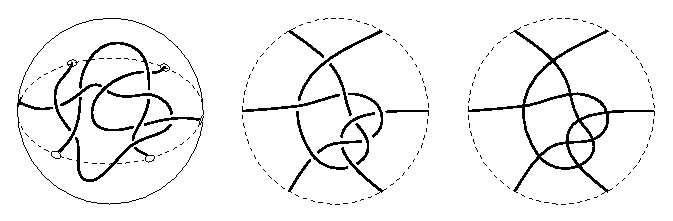
\includegraphics[scale = 0.7]{c/tangle-diagram-projection.eps}
		\end{figure}

		\begin{definition}
			\label{definition:tangle-equiv}
			$k$-танглы $T_1$ и $T_2$ называются эквивалентными, если существует изотопия $B^3$, сохраняющая границу
			неподвижной, которая переводит $T_1$ в $T_2$.
		\end{definition}
	\end{frame}

%	\begin{frame}
%		\frametitle{Основные определения}
%
%		\begin{definition}
%			$k$-танглы $T_1$ и $T_2$ называются слабо эквивалентными, если существует изотопия $B^3$ (не обязательно
%			сохраняющая границу неподвижной) которая переводит $T_1$ в $T_2$.
%		\end{definition}
%
%		\begin{figure}[ht]
%			\centering
%			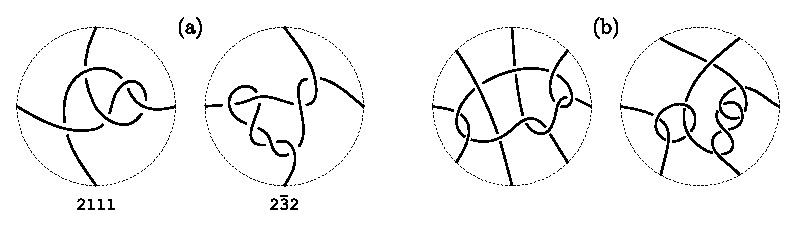
\includegraphics[scale = 0.7]{tangles-example.eps}
%			\caption{$2$-танглы (a), $k$-танглы в общем случае (b)}
%		\end{figure}
%	\end{frame}

	\begin{frame}
		\frametitle{Основные определения}

		\begin{definition}
			Диаграмма (проекция) $k$-тангла называется составной, если строго внутри граничной окружности существует замкнутая
			гладкая несамопересекающаяся кривая, которая трансверсально пересекает диаграмму ровно в двух точках и содержит
			внутри как минимум один перекресток. В противном случае диаграмма называется простой.
		\end{definition}

		\begin{figure}[H]
			\centering
			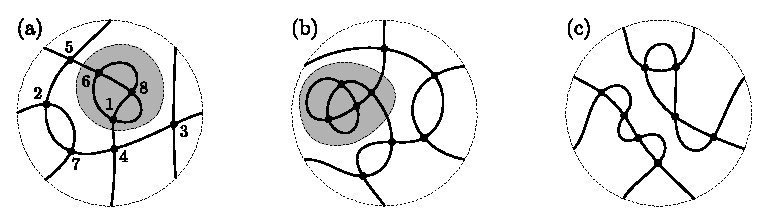
\includegraphics[scale = 0.7]{c/composite-non-connected-projections.eps}
			\caption{Составные (a, b) и несвязные (c) проекции}
		\end{figure}

		\begin{definition}
			Диаграмма (проекция) называется связной, если граф, ребрами которого являются ребра диаграммы (проекции), а
			вершинами --- вершины и концы диаграммы (проекции), является связным.
		\end{definition}
	\end{frame}

	\begin{frame}
		\frametitle{Tait flyping conjecture}

		\begin{figure}[ht]
			\centering
			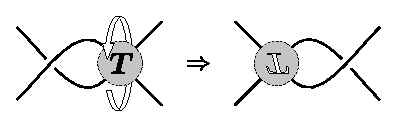
\includegraphics{c/flype.eps}
			\caption{Flype}
		\end{figure}
	\end{frame}

	\begin{frame}
		\frametitle{Операции с проекциями}

		\begin{figure}[ht]
			\centering
			$\putGen{6} {}\to{} \putGen{5} {}\to{} \putGen{4} {}\to{} \putGen{3} {}\to{} \putGen{2} {}\to{} \putGen{1}$
		\end{figure}

		\begin{theorem}
			В любой связной простой проекции $k$-тангла, содержащей более одного перекрестка, можно удалить пограничный
			перекресток так, чтобы получившаяся в результате проекция была простой и связной.
		\end{theorem}
	\end{frame}

	\begin{frame}
		\frametitle{Доказательство}

		Простота любой получающейся проекции очевидна. Осталось доказать возможность получения связной проекции, показав,
		что среди пограничных перекрестков найдется не являющийся точкой сочленения проекции. Точка сочленения --- перекресток,
		через которую можно провести хорду (гладкую несамопересекающуюся кривую, только начало и конец которой лежат на граничной
		окружности), которая больше нигде с проекцией не пересекается, и с обеих сторон от которой есть перекрестки.
		\begin{figure}[H]
			\centering
			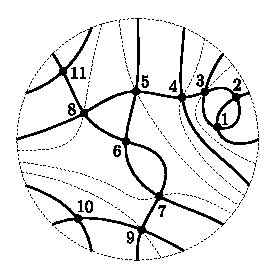
\includegraphics[scale = 1]{c/cutpoints-proof.eps}
		\end{figure}
	\end{frame}

	\begin{frame}
		\frametitle{Инвариант}

		\begin{block}{root-code$(P, (v, e, f))$}
		{
			\footnotesize
			\begin{algorithmic}[H]
				\STATE $A \leftarrow \{\}$
				\STATE $free \leftarrow 2$

				\STATE $Q \leftarrow \{v\}$
				\STATE $number[v] \leftarrow 1$
				\STATE $incoming[v] \leftarrow e$

				\WHILE{$Q \neq \varnothing$}
					\STATE $u \leftarrow head[Q]$
					\STATE $dequeue(Q)$

					\FOR{(для) всех ребер $(u, w) \in P$ в порядке, заданном $f$, начиная с $incoming[u]$}
						\IF{$w$ --- конец диаграммы}
							\STATE $code \leftarrow 0$
						\ELSE
							\IF{$number[w]$ не определен}
								\STATE $number[w] \leftarrow free$
								\STATE $free \leftarrow free + 1$
								\STATE $enqueue(Q, w)$
							\ENDIF
							\STATE $code \leftarrow number[w]$
						\ENDIF

						\STATE $push(A, code)$
					\ENDFOR
				\ENDWHILE

				\RETURN $A$
			\end{algorithmic}
		}
		\end{block}
	\end{frame}

	\begin{frame}
		\frametitle{Пример}

		\begin{figure}[ht]
			\centering
			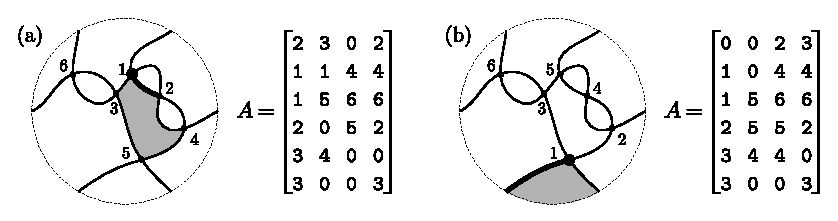
\includegraphics[scale = 0.7]{c/rcode-example.eps}
			\caption{Примеры вычисления root-code\label{figure:rcode-example}}
		\end{figure}
	\end{frame}


	\begin{frame}
		\frametitle{Дерево проекций}

		\begin{definition}
			Пусть $I$ --- проекция тангла, состоящая из единственного пререкрестка. Определим на множестве простых связных
			прекций $k$-танглов отображение $prev(T)$ следующим образом:
			\begin{itemize}
				\item
				$prev(I) = \varnothing$

				\item
				Для всех остальных $prev(T)$ будет являться результатом удаления из $T$ пограничного перекрестка $v$, не
				являющегося точкой сочленения, такого что root-code($T$, $v$) лексикографически минимален среди всех подобных
				перекрестков.
			\end{itemize}
		\end{definition}

		\begin{itemize}
			\item
			$prev(T)$ определено на всем множестве простых связных проекций $k$-танглов

			\item
			$prev(T)$ однозначно

			\item
			$prev(T)$ обладает полуинвариантом --- числом перекрестков
		\end{itemize}
	\end{frame}

	\begin{frame}
		\frametitle{Дерево проекций}

		\begin{figure}[ht]
			\centering
			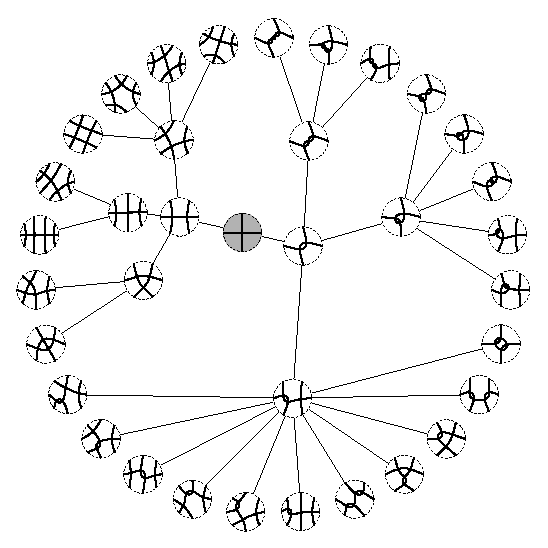
\includegraphics[scale = 0.9]{c/genealogical-tree.eps}
		\end{figure}
	\end{frame}

	\begin{frame}
		\frametitle{Алоритм}

		\begin{block}{DFS(T)}
		{
			\footnotesize
			\begin{algorithmic}[H]
				\algsetup{linenosize=\small, linenodelimiter=.}
				\PRINT $T$
				\IF{$crossings[T] = n$}
					\RETURN
				\ENDIF

				\STATE $list \leftarrow \varnothing$
				\FOR{(для) всех возможных результатов $R$ приклеивания перекрестка $v$ к $T$}
					\IF{$R$ --- простая}
						\IF{$prev(R) = T$}
							\STATE $r \leftarrow $ root-code($R$, $v$)
							\IF{ {\bf not} $contains(list, r)$}
								\STATE DFS($R$)
								\STATE $add(list, r)$
							\ENDIF
						\ENDIF
					\ENDIF
				\ENDFOR
			\end{algorithmic}
		}
		\end{block}
	\end{frame}




	\begin{frame}
		\frametitle{Теорема о пересекающихся танглах}

		Под словом ``тангл'' ниже будет подразумеваться простую связную диаграмму альтернированного $2$-тангла.

		\begin{theorem}
			\label{theorem:tangle-decomp-th}
			Пусть у нас есть два связных тангла $A$ и $B$, содержащиеся в какой-то простой альтернированной диаграмме
			тангла или зацепления $D$. При этом $A\setminus B\neq\varnothing$, $B\setminus A\neq\varnothing$
			и $A\cap B\neq\varnothing$. Тогда $A\setminus B$, $B\setminus A$, $A\cap B$ и $A\cup B$ --- также связные
			танглы, а $A\cup B$ представим в виде:

			\begin{figure}[H]
				\centering
				\includegraphics{tangle-decomp-theorem.eps}
			\end{figure}
		\end{theorem}
	\end{frame}

	\begin{frame}
		\frametitle{Доказательство}

		\begin{figure}[H]
			\centering
			\includegraphics[scale = 0.8]{tangle-decomp-proof.eps}
		\end{figure}

		\begin{equation}
			\label{equation:a_relation}
			a + c + e + f = 4
		\end{equation}
		\begin{equation}
			\label{equation:b_relation}
			b + c + d + f = 4
		\end{equation}

		\begin{equation}
			\label{equation:ab_relation}
			d + e + c \ge 4
		\end{equation}
		\begin{equation}
			\label{equation:all_relation}
			a + b + c \ge 4
		\end{equation}
		\begin{equation}
			\label{equation:amb_relation}
			a + d + f \ge 4
		\end{equation}
		\begin{equation}
			\label{equation:bma_relation}
			b + e + f \ge 4
		\end{equation}
	\end{frame}

	\begin{frame}
		\frametitle{Доказательство}

		\begin{figure}[H]
			\centering
			\includegraphics[scale = 0.8]{tangle-decomp-proof.eps}
		\end{figure}

		Складывая попарно (\ref{equation:a_relation}) и (\ref{equation:b_relation}),
		(\ref{equation:ab_relation}) и (\ref{equation:all_relation}),
		(\ref{equation:amb_relation}) и (\ref{equation:bma_relation}), получаем соответственно:
		\[a + b + d + e + 2c + 2f = 8\]
		\[a + b + d + e + 2c \ge 8\]
		\[a + b + d + e + 2f \ge 8\]
		Отсюда следует, что $c = f = 0$, а все нестрогие неравенства на самом деле являются равенствами. В результате
		получаем систему линейных уравнений на $a$, $b$, $d$ и $e$, единственным решением которой является
		$a = b = d = e = 2$. Завершим доказательство, заметив, что для связности $A\setminus B$, $B\setminus A$ и
		$A\cap B$ достаточно простоты $D$.
	\end{frame}

	\begin{frame}
		\frametitle{Разложение на $2$-танглы}

		\begin{figure}[ht]
			\centering
			$$\putDC{1} \qquad \Rightarrow \qquad \putDC{2}$$
		\end{figure}

		Требования к разложению: \\
		$v \in T \rightarrow S(v) \subset T$
		\begin{itemize}
			\item $v \in S(v)$
			\item $\forall R \subset T$, где $R$ --- $2$-тангл, $v \in R \Rightarrow R \subset S(v)$
			\item $\forall u, u \in S(v) \Leftrightarrow S(u) = S(v)$
		\end{itemize}
	\end{frame}

	\begin{frame}
		\frametitle{Обобщение инварианта}

		\begin{block}{root-code-decomp$(P, (v, e, f))$}
		{
			\footnotesize
			\begin{algorithmic}[H]
				\STATE $A \leftarrow \{\}$
				\STATE $free \leftarrow 2$

				\STATE $Q \leftarrow \{v\}$
				\STATE $number[v] \leftarrow 1$
				\STATE $incoming[v] \leftarrow e$

				\WHILE{$Q \neq \varnothing$}
					\STATE $u \leftarrow head[Q]$
					\STATE $dequeue(Q)$

					\STATE \textcolor{red}{$push(A, tangle(u))$}

					\FOR{(для) всех ребер $(u, w) \in P$ в порядке, заданном $f$, начиная с $incoming[u]$}
						\IF{$w$ --- конец диаграммы}
							\STATE $code \leftarrow 0$
						\ELSE
							\IF{$number[w]$ не определен}
								\STATE $number[w] \leftarrow free$
								\STATE $free \leftarrow free + 1$
								\STATE $enqueue(Q, w)$
							\ENDIF
							\STATE $code \leftarrow number[w]$
						\ENDIF

						\STATE $push(A, code)$
					\ENDFOR

					\STATE \textcolor{red}{$push(A, orientation(u, incoming[u], f))$}
				\ENDWHILE

				\RETURN $A$
			\end{algorithmic}
		}
		\end{block}
	\end{frame}

	\begin{frame}
		\frametitle{$2$-танглы}

		\begin{theorem}
			Если для какого-то $2$-тангла $T$ не существует корректного разложения на $2$-танглы, то $T$ представим в виде прямой
			суммы двух или более $2$-танглов.
			\begin{figure}[H]
				\centering
				\includegraphics[scale = 0.5]{tangle-sum.eps}
			\end{figure}
		\end{theorem}
		\begin{proof}
			Если для $T$ не существует разложения на $2$-танглы, то в $T$ есть перекресток $v$ и собственные $2$-подтанглы $A$ и $B$
			такие, что $v \in A$, $v \in B$, $A\setminus B\neq\varnothing$, $B\setminus A\neq\varnothing$ и не существует такого
			собственного подтангла $T$, чтобы он содержал $A$ и $B$. Но $A \cup B$ --- $2$-тангл, следовательно $T = A \cup B$.
		\end{proof}
	\end{frame}

	\begin{frame}
		\frametitle{$2$-танглы}

		\begin{figure}[ht]
			\centering
			\includegraphics[scale = 0.5]{one-side-crossings.eps}
		\end{figure}

		
		\begin{center}
			У одиночного перекрестка минимальный номер.
		\end{center}

		\begin{table}[ht]
			\caption{Правила сборки прямых сумм\label{table:sums-rules}}
			\centering
			\begin{tabular}{cm{22mm}l}
				\hline
				1 & \includegraphics[scale = 0.5]{alternating-build-4-case-1.eps} & --- принять \\
				2 & \includegraphics[scale = 0.5]{alternating-build-4-case-2.eps} & --- принять \\
				3 & \includegraphics[scale = 0.5]{alternating-build-4-case-3.eps} & --- сравнить по root-code-decomp \\
				4 & \includegraphics[scale = 0.5]{alternating-build-4-case-4.eps} & --- нарушается положение перекрестков \\
				5 & \includegraphics[scale = 0.5]{alternating-build-4-case-5.eps} & --- нарушается положение перекрестков \\
				6 & \includegraphics[scale = 0.5]{alternating-build-4-case-6.eps} & --- не бывает \\
				7 & \includegraphics[scale = 0.5]{alternating-build-4-case-7.eps} & --- принять \\
				8 & \includegraphics[scale = 0.5]{alternating-build-4-case-8.eps} & --- не бывает \\
				\hline
			\end{tabular}
		\end{table}

	\end{frame}

	\begin{frame}
		\frametitle{Результаты}

		\begin{figure}[H]
			\begin{minipage}{0.49\linewidth}
				\center{ 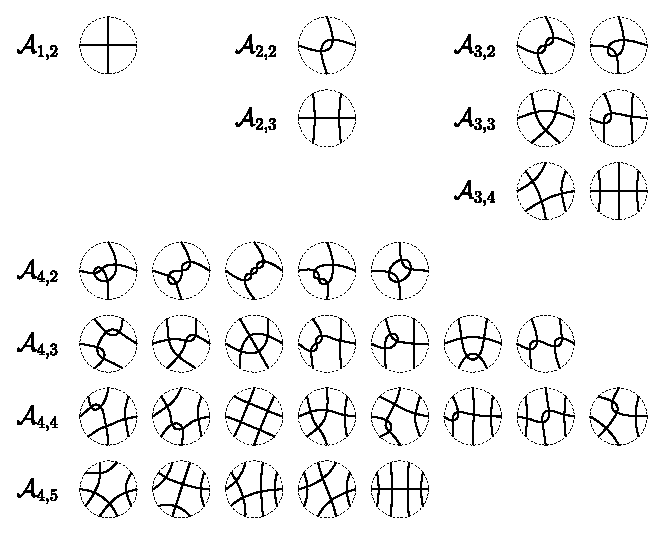
\includegraphics[scale = 0.4]{c/alternating-tangles-1-4.eps} }
			\end{minipage}
			\hfill
			\begin{minipage}{0.49\linewidth}
				\center{ 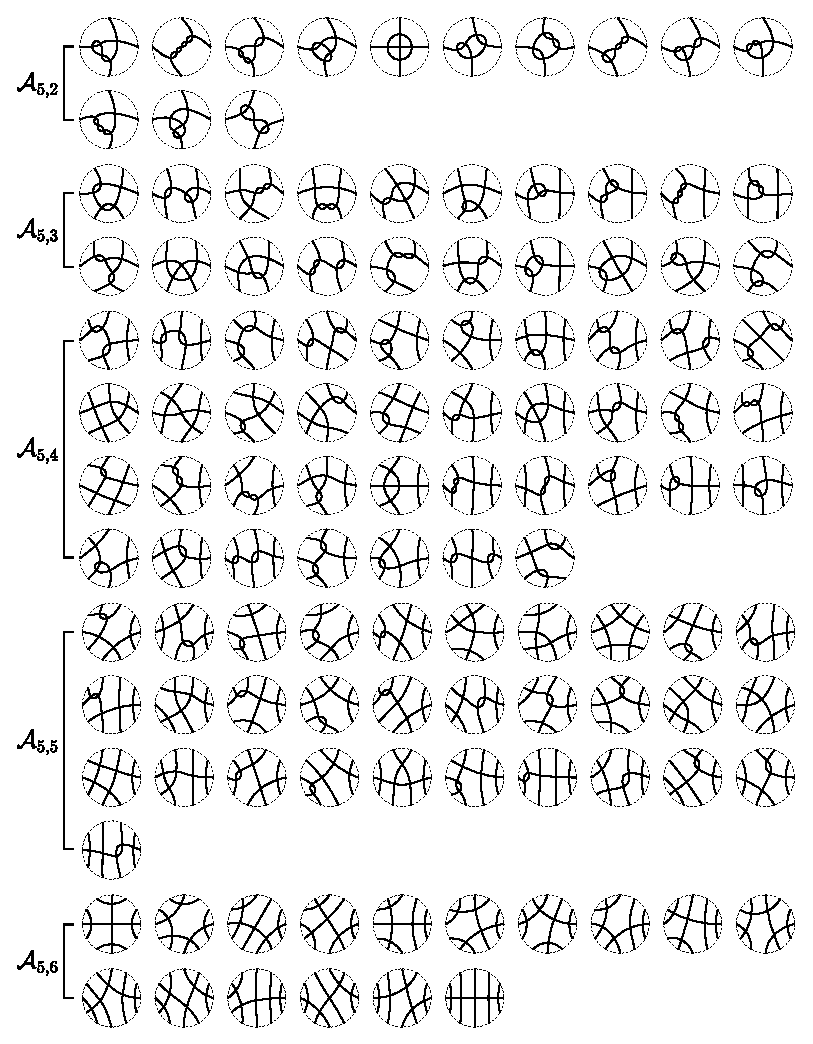
\includegraphics[scale = 0.4]{c/alternating-tangles-5.eps} }
			\end{minipage}
		\end{figure}
	\end{frame}

	\begin{frame}
		\frametitle{Результаты}

		\begin{table}[ht]
		{
			\tiny
			\centering
			\begin{tabular}{|c||r|r|r|r|r|r|r|r|r|r|r|r|}
			\hline
			$k$\textbackslash $n$
			    & 1 & 2 & 3 &  4 &   5 &   6 &      7 &       8 &        9 &          10 &           11 \\
			\hline\hline
			2   & 1 & 1 & 2 &  5 &  13 &  36 &    111 &     373 &   1\,362 &      5\,378 &      22\,807 \\
			3   & . & 1 & 2 &  7 &  20 &  77 &    276 &  1\,135 &   4\,823 &     21\,734 &     101\,307 \\
			4   & . & . & 2 &  8 &  37 & 157 &    687 &  3\,052 &  13\,981 &     65\,797 &     317\,506 \\
			5   & . & . & . &  5 &  31 & 209 & 1\,128 &  5\,986 &  30\,556 &    155\,964 &     795\,918 \\
			6   & . & . & . &  . &  16 & 161 & 1\,294 &  8\,528 &  51\,475 &    294\,366 &  1\,637\,855 \\
			7   & . & . & . &  . &   . &  60 &    840 &  8\,206 &  62\,895 &    428\,254 &  2\,702\,902 \\
			8   & . & . & . &  . &   . &   . &    261 &  4\,702 &  52\,815 &    460\,189 &  3\,475\,551 \\
			9   & . & . & . &  . &   . &   . &      . &  1\,243 &  26\,753 &    341\,878 &  3\,327\,424 \\
			10  & . & . & . &  . &   . &   . &      . &       . &   6\,257 &    155\,593 &  2\,221\,544 \\
			11  & . & . & . &  . &   . &   . &      . &       . &        . &     32\,721 &     916\,595 \\
			12  & . & . & . &  . &   . &   . &      . &       . &        . &           . &     175\,760 \\
			\hline
			все & 1 & 2 & 6 & 25 & 117 & 700 & 4\,597 & 33\,225 & 250\,917 & 1\,961\,874 & 15\,695\,169 \\
			\hline
			\end{tabular}
		}
		\end{table}

		Преимущества:
		\begin{itemize}
			\item Не нужна хеш-таблица.
			\item Легко распараллелить.
			\item Легко обобщить.
		\end{itemize}
	\end{frame}

\end{document}
